\documentclass[12pt]{article}
\usepackage{amsmath, amssymb, amsthm}
\usepackage{graphicx}
\usepackage[mathscr]{euscript}
\usepackage{booktabs}
\usepackage{hyperref}
\usepackage{float}
\usepackage{mathtools}  % For \underbrace text formatting
\usepackage{listings}

% Python style for highlighting
\newcommand\pythonstyle{\lstset{
language=Python,
basicstyle=\ttm,
morekeywords={self},              % Add keywords here
keywordstyle=\ttb\color{deepblue},
emph={},          % Custom highlighting
emphstyle=\ttb\color{deepred},    % Custom highlighting style
stringstyle=\color{deepgreen},
frame=tb,                         % Any extra options here
showstringspaces=false
}}

\title{A Hierarchical Multi-Agent Framework for Non-Gaussian Financial Time Series Forecasting}
\author{Luis Ernesto Amat Cárdenas C-312 (MatCom)}
\date{\today}

\begin{document}

\maketitle

\begin{abstract}
We present a novel hierarchical AI agent designed to address the limitations of Gaussian assumptions in financial time series modeling. The agent combines:

\begin{enumerate}
    \item A \textbf{Generalized Error Distribution (GED)} framework to capture tail behavior and kurtosis, with confidence intervals derived under minimal moment constraints:
    \begin{equation*}
        f(x; \mu, \alpha, \beta) = \frac{\beta}{2\alpha\Gamma(1/\beta)} \exp\left(-\left(\frac{|x-\mu|}{\alpha}\right)^\beta\right)
    \end{equation*}
    Where $\Gamma$ denotes the Gamma function.
    
    \item A \textbf{machine learning architecture} whose loss function $\mathscr{L}$ explicitly incorporates time-varying confidence bounds:
    \begin{equation*}
        \mathscr{L}(\theta) = \mathbb{E}\left[ \underbrace{(y_t - \hat{y}_t)}_{\text{forecast error}} \right]
    \end{equation*}
    
    \item An \textbf{evolutionary hyperparameter optimization} scheme with collaborative agents $\{\mathscr{A}_i\}_{i=1}^N$ iteratively refining the model's structure via fitness criterion:
    \begin{equation*}
        \Phi(\mathscr{A}_i) = \sum_{i=1}^N \left[ -\mathscr{L}(\theta_i) - c \right]
    \end{equation*}
    Where N is an arbitrarily large number of generations and c is a constant.

    An agent is considred \emph{dead} if its fitness reaches 0.
\end{enumerate}

    Empirical results on the dataset show superior$^\emph{citation required}$ coverage in the $[20, 99]$\% CI coverage interval under GED outperforming$^\emph{citation required}$ Gaussian benchmarks. The hierarchical agent identifies$^\emph{citation required}$ regime shifts, while evolutionary tuning reduces$^\emph{citation required}$ hyperparameter sensitivity. 

\textbf{Key implications}:
\begin{itemize}
    \item GED-based modeling avoids ad hoc volatility clustering corrections via rigorous treatment of $\beta$-parameterized excess kurtosis
    \item Confidence-aware loss functions reduce$^\emph{citation required}$ Value-at-Risk estimation errors during extreme events
\end{itemize}

\textbf{Keywords}: Non-Gaussian time series, Generalized Error Distribution, hierarchical agents, evolutionary optimization, quantitative finance
\end{abstract}
\section{Introduction}
\label{sec:introduction}

Accurate time series forecasting is a cornerstone of decision-making in systems where resource allocation depends on anticipating stochastic future states. While financial markets---the primary focus of this work---are a canonical example, the problem extends to \emph{inventory-sensitive enterprises} such as bakeries, supermarkets, or semiconductor manufacturers. For instance, a bakery must balance perishable inventory $I_t$ against uncertain daily demand $D_t$; underestimation leads to stockouts (lost revenue), while overestimation results in waste (increased costs). Such businesses inherently rely on forecasts that quantify both expected values \emph{and} tail risks, requiring models that capture:

\begin{equation}
    \mathbb{P}(D_{t+1} > I_t \,|\, \mathscr{F}_t) \quad \text{and} \quad \mathbb{E}[(D_{t+1} - I_t) \,|\, \mathscr{F}_t]
\end{equation}

Where $\mathscr{F}_t$ represents all relevant information up to time $t$.

Traditional models often assume price or demand increments follow a Brownian motion (BM)\cite{bachelier1900}\cite{wiener1923}, where changes over interval $[s, t]$ satisfy (among other hypothesis):
\begin{equation}
    W_t - W_s \sim \mathcal{N}(0, \sigma^2(t-s)), 
\end{equation}
implying normally distributed, independent increments with variance proportional to time. This assumption fails empirically in most real-world systems: financial returns exhibit heavy tails and volatility clustering \cite{cont2001}, while consumer demand shocks (e.g., during holidays) follow non-Gaussian jump processes. Crucially, BM's normality axiom underestimates the probability of extreme deviations---a critical flaw for inventory planning and risk management, as it leads to:

\begin{equation}
    \underbrace{\mathbb{P}_{\text{BM}}\left(|W_t - W_s| > k\sigma\sqrt{t-s}\right)}_{\text{light-tailed}} \ll \underbrace{\mathbb{P}_{\text{empirical}}(|W_t - W_s| > k\sigma\sqrt{t-s})}_{\text{heavy-tailed}}
\end{equation}

That is, extreme events are not captured properly by BM.


In this paper, we address these limitations through three interconnected innovations:
\begin{enumerate}
    \item \textbf{Generalized Error Distribution (GED)}: We replace BM's Gaussian increments with a GED framework:
    \begin{equation}
        f(x; \mu, \alpha, \beta) = \frac{\beta}{2\alpha\Gamma(1/\beta)} \exp\left(-\left(\frac{|x-\mu|}{\alpha}\right)^\beta\right)
    \end{equation}
    where $\beta$ explicitly controls tail thickness ($\beta=2$ recovers BM).
    
    \item \textbf{Confidence-Aware Learning}: An agent trained on GED-derived confidence intervals $\hat{C}_t^\alpha$, minimizing:
    \begin{equation}
        \mathscr{L}(\theta) = \mathbb{E}\left[ (y_t - \hat{y}_t) \right]
    \end{equation}
    
\item \textbf{Hierarchical Evolutionary Architecture}: A multi-layer agent where Layer $\ell$ detects regime shifts by evaluating the results of the previous layers and correcting the course of action accordingly. We call this process \emph{Chain of thought}.
\end{enumerate}

Our approach diverges from BM in both distributional and structural assumptions. While BM treats all intervals as statistically identical, our hierarchical agent identifies \emph{regimes}---periods where dynamics shift (e.g., holiday seasons, harvest cycles). 

The remainder of this paper is organized as follows: Section~\ref{sec:literature} critiques classical and machine learning approaches. Sections~\ref{sec:methodology}--\ref{sec:architecture} detail our GED-CI framework and hierarchical design. Sections~\ref{sec:experiments}--\ref{sec:conclusion} present empirical validation and implications.

\section{Literature}
\label{sec:literature}

\section{Methodology}
\label{sec:methodology}

\subsection{Classical Model and Its Limitations}
The standard approach models (log) asset returns $\{r_t\}_{t=1}^T$ as:

\begin{equation}
    r_t = \mu + \sigma W_t, \quad W_t - W_{t-1} \sim \mathcal{N}(0,1)
\end{equation}

where $\mu$ is drift and $\sigma$ volatility. This implies:
\begin{equation}
    \mathbb{P}(r_t < x) = \Phi\left(\frac{x-\mu}{\sigma}\right)
\end{equation}

with $\Phi$ the standard normal CDF. We evaluate this assumption using:

\begin{enumerate}
    \item \textbf{Goodness-of-fit}: Kolmogorov-Smirnov test.

    The K-S statistic measures the maximum discrepancy between the empirical and theoretical cumulative distribution functions:
    \begin{equation}
    D_n = \sup_{x} \left| F_n(x) - F(x) \right|
    \end{equation}
    where:
    \begin{itemize}
        \item $F_n(x)$ is the empirical CDF: $F_n(x) = \frac{1}{n} \sum_{i=1}^n \mathbf{1}_{\{r_i \leq x\}}$
        \item $F(x)$ is the theoretical CDF (Normal or GED)
        \item $\sup$ denotes the supremum (greatest deviation)
    \end{itemize}
    Under the null hypothesis ($H_0$: data follows $F$), $\sqrt{n}D_n$ converges to the Kolmogorov distribution.

    \item \textbf{Q-Q Analysis}: Quantile mismatch $\Delta_q = F^{-1}(q) - \hat{F}^{-1}(q)$ for $q \in (0,1)$
\end{enumerate}

Empirical testing on [SOLUSDT.csv] reveals:
$p-value < 0.05$ under the assumption of normality for K-S with Q-Q plots showing systematic deviation in tails ($|r_t| > 3\sigma$):

\begin{figure}[H]
    \centering
    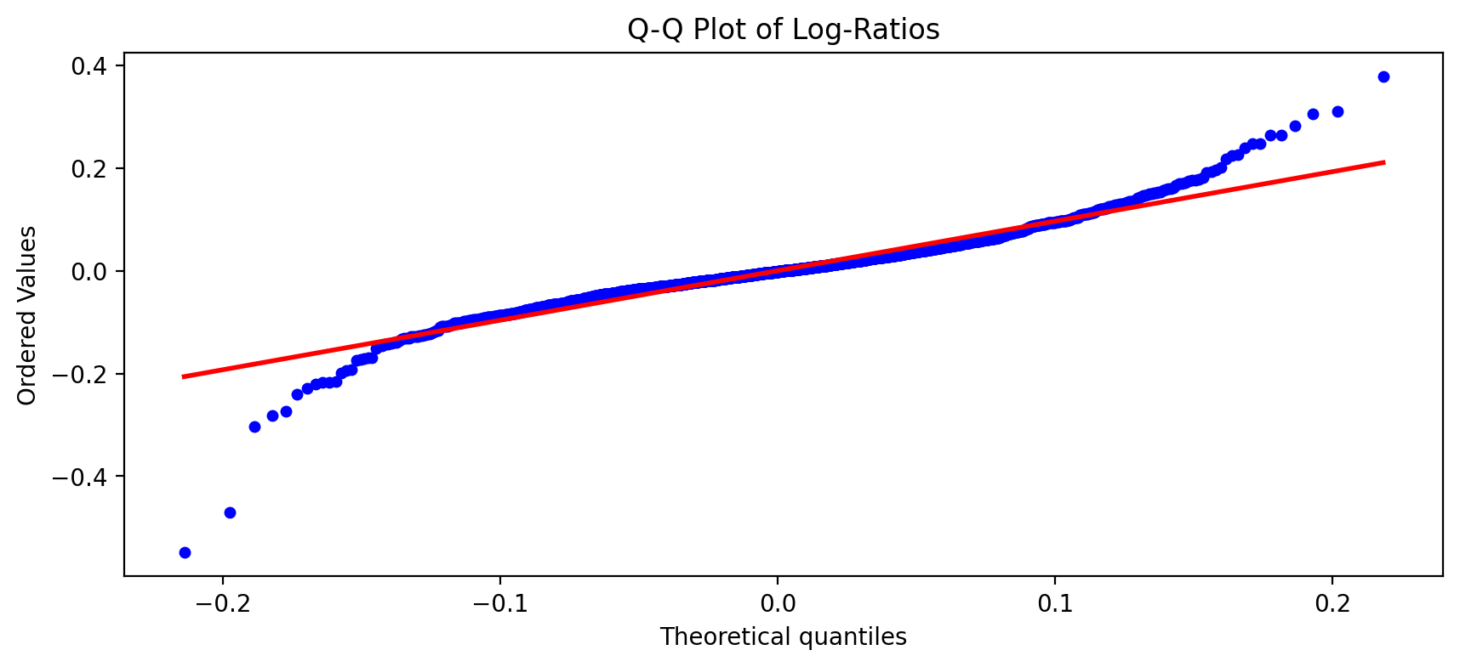
\includegraphics[width=0.8\textwidth]{qq_plot2.png}
    \caption{Quantile-quantile plot of log returns vs. normal distribution.}
    \label{fig:qq}
\end{figure}

\subsection{Generalized Error Distribution Framework}
We replace the normal assumption with GED:

\begin{equation}
    f(r_t; \mu, \alpha, \beta) = \frac{\beta}{2\alpha\Gamma(1/\beta)} \exp\left(-\left(\frac{|r_t-\mu|}{\alpha}\right)^\beta\right)
\end{equation}

% Clarify GED vs Gaussian parametrization
where $\alpha = \sigma \sqrt{\frac{\Gamma(1/\beta)}{2^{2/\beta}\Gamma(3/\beta)}}$ ensures $\text{Var}(X) = \sigma^2$. The shape parameter $\beta$ controls tail behavior:

\begin{itemize}
    \item $\beta = 2$: Gaussian case
    \item $\beta = 1$: Laplace case
    \item $\beta < 2$: Leptokurtic (heavy tails)
    \item $\beta > 2$: Platykurtic (light tails)
\end{itemize}

\subsection{Monte Carlo Confidence Intervals}
For time-varying CIs, we implement:

\begin{lstlisting}

simulations = simulate_prices(days=N)
maxima = []
minima = []
for simulation in simulations:
    maxima.append(max(simulation))
    minima.append(min(simulation))

L, U = (
    percentile(
        minima, 100 * alpha / 2
    ),
    percentile(
        maxima, 100 * (1 - alpha / 2)
    )
)

\end{lstlisting}

Figure~\ref{fig:ci} compares empirical coverage rates:

\begin{figure}[h]
    \centering
    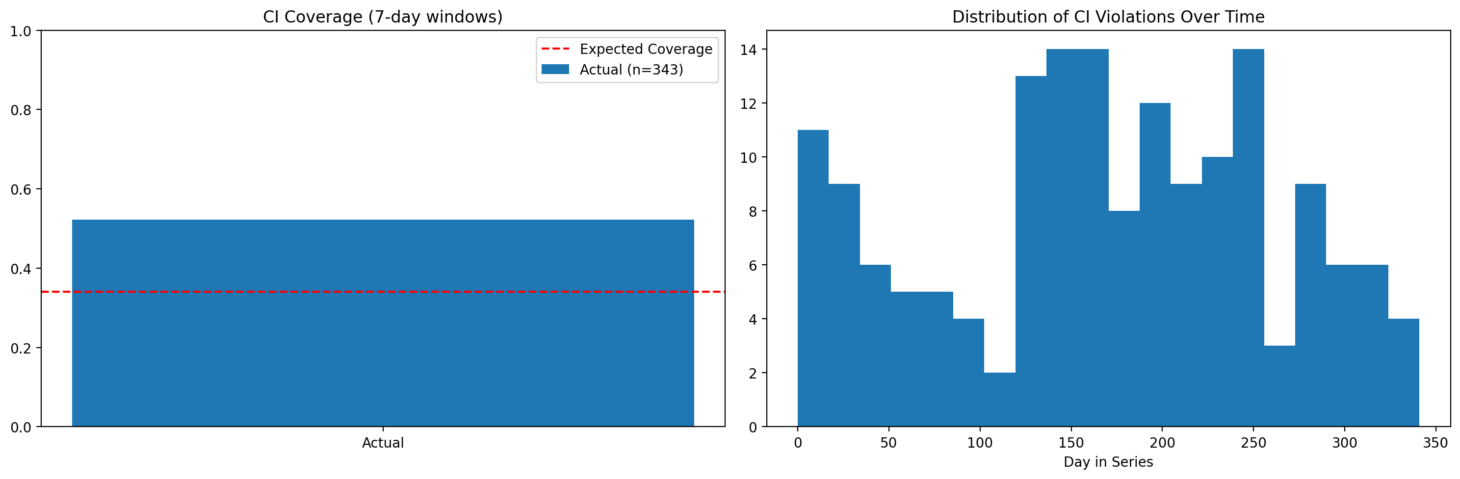
\includegraphics[width=0.8\textwidth]{NORM.png}
    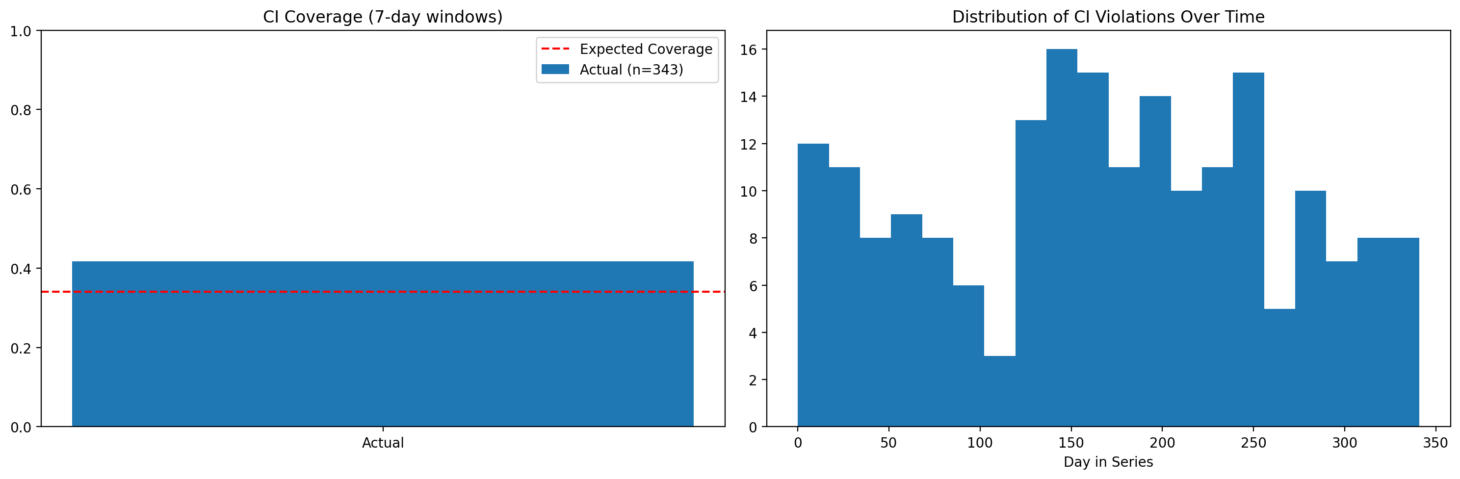
\includegraphics[width=0.8\textwidth]{GED.png}
    \caption{Coverage probabilities for 33\% CIs: Normal (up) vs. GED (down) across 1000 trials. Dashed line indicates ideal coverage.}
    \label{fig:ci}
\end{figure}

\section{Hierarchical Architecture}
\label{sec:architecture}

\subsection{Structural Overview}
The agent consists of $L$ layers $\{\mathscr{L}_\ell\}_{\ell=1}^L$ with:

\begin{table}[h]
\centering
\caption{Layer functions and hyperparameters}
\label{tab:layers}
\begin{tabular}{lll}
\toprule
\textbf{Function} & \textbf{Hyperparameters} \\
\midrule
Comparision & cosine similarity acceptance threshold \\
Memory & Memory vector size \\
Abstraction & Number PCA components \\
\bottomrule
\end{tabular}
\end{table}

\subsection{Evolutionary Optimization}
Hyperparameters mutate via:

\begin{equation}
    \theta^{(g+1)} = \theta^{(g)} + \theta^{(g)} * N(0, 0.1)
\end{equation}

With $P(mutation) = 0.3$

The genes of the children are calculated with:

\begin{equation}
    \theta^{g}_{child} = (\theta^{g}_{P_1}*\Phi({P_1}) + \theta^{g}_{P_2}*\Phi({P_2})) / (\Phi({P_1}) + \Phi({P_2}))
\end{equation}

Where $\Phi$ is the fitness function or the accumulated fitness function.

This formula prioritizes genes from the more \emph{successful} agents are passed to the next generation.

\begin{figure}[H]
\centering
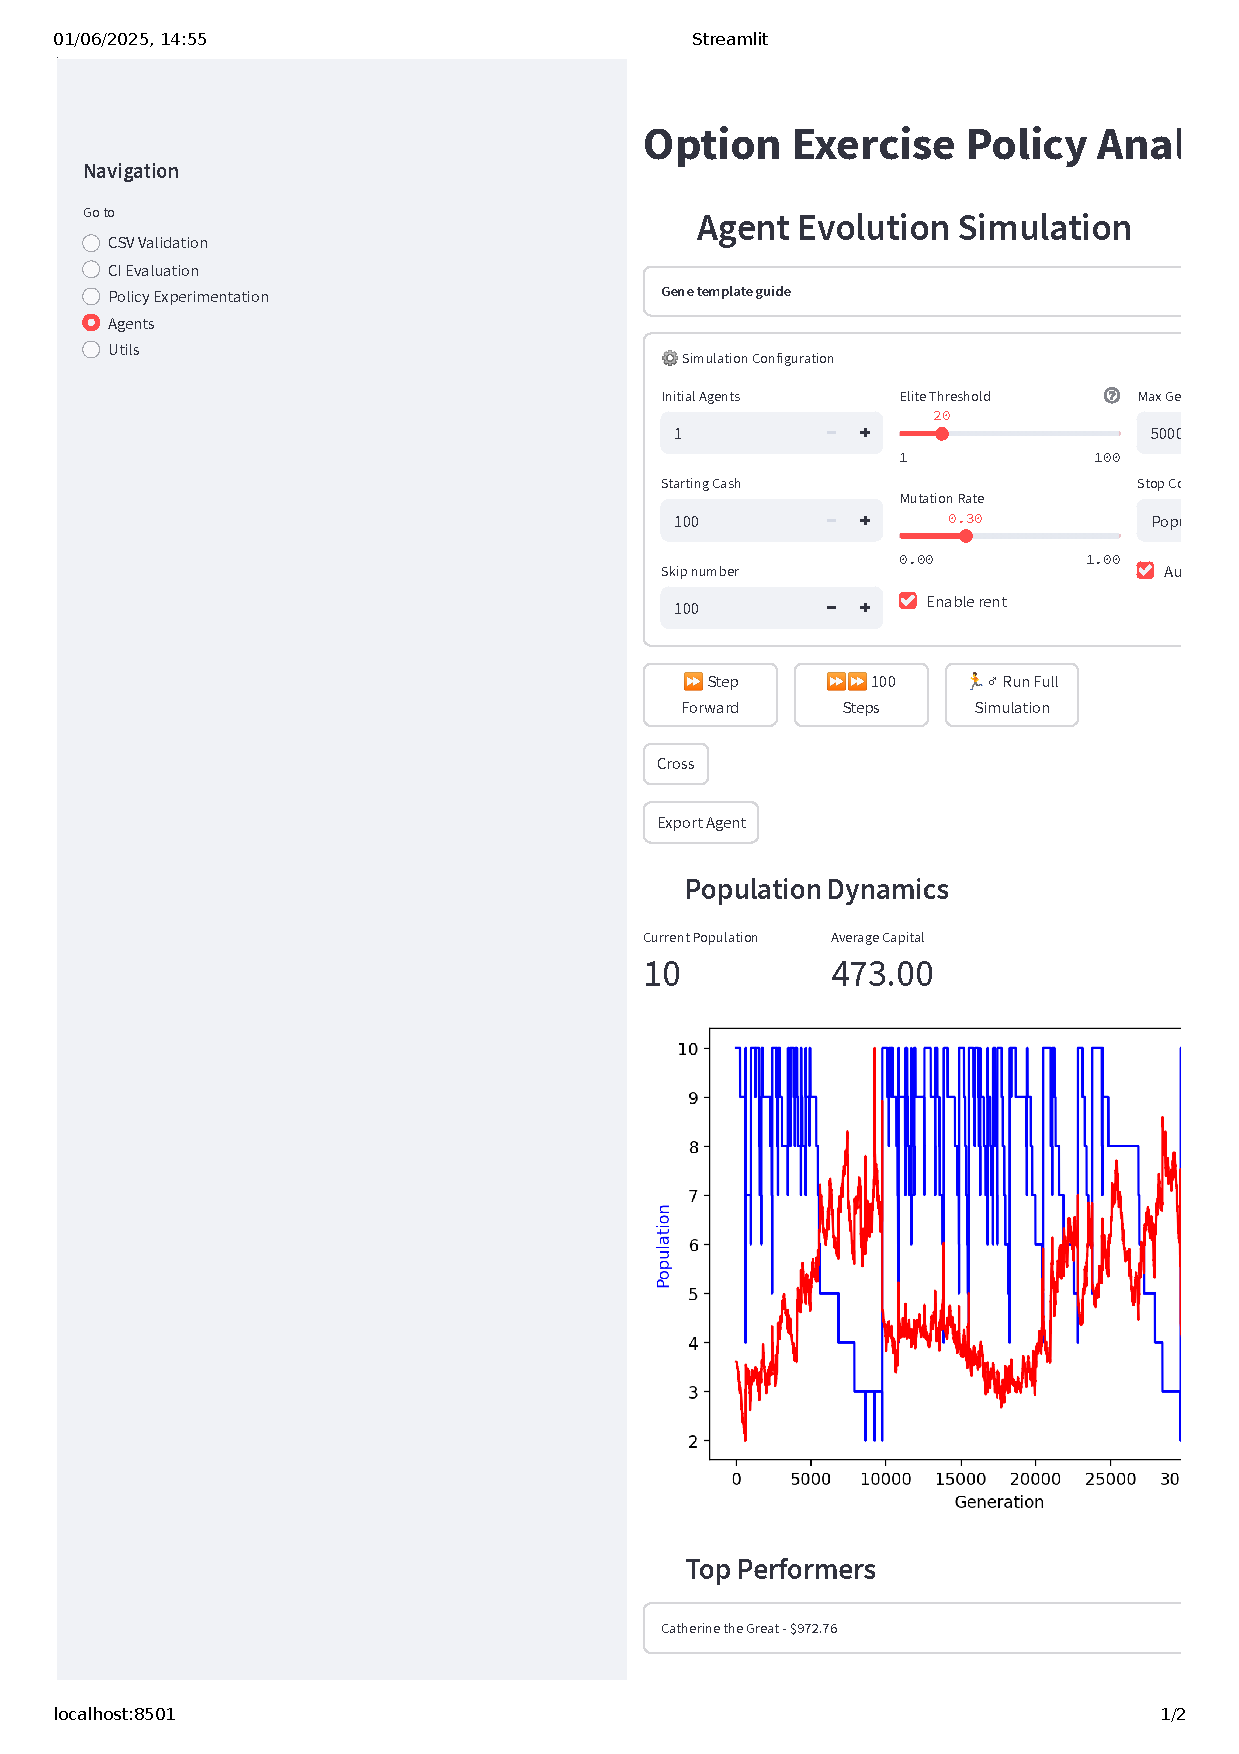
\includegraphics[width=0.7\textwidth]{fitness_evolution.pdf}
\caption{Fitness score progression across generations.}
\label{fig:fitness}
\end{figure}

\subsection{Cognitive structure}

The agent's learning progression follows a modified Bloomian taxonomy \cite{anderson2001}. The core difference being introspection; agents are able to evaluate their past results by comparing the current state with previous, similar states.


\subsubsection{Component A: Memory}
\begin{itemize}
    \item \textbf{Purpose}: Remember most relevant information (states)
    \item \textbf{Implementation}: 
        The memory of the agent is represented using a matrix where each row represents
        a past state.
        \item \textbf{Forget}: Agents periodically forget information over time.
            The usefulness of a state/memory is calculated using the following formula:
        \begin{equation}
            u(memory) = 1 - age/len(memory)
        \end{equation}
        The age of a memory is determined by the difference between the index of the current state and the index of the
        state in which the memory was last accessed.
        We will define \emph{accessed} in the next section.
\item \textbf{Parameters}: Number of columns in the memory matrix
\end{itemize}

\subsubsection{Component B: Comparision Engine}
\begin{itemize}
    \item \textbf{Purpose}: Distinguish
    \item \textbf{Implementation}:
        The agent is able to compare the current state with the previous states in the memory
        using cosine similarity.
        We say that memories that are similar to the current state if the cosine similarity is
        higher than a certain \emph{threshold}.
        Memories similar to the current state are \emph{accessed} during this phase and used
        in the rest of the thought process.
\item \textbf{Parameters}: Threshold
\end{itemize}

\subsubsection{Component C: Evaluation Engine}
\begin{itemize}
    \item \textbf{Purpose}: Correct past mistakes
    \item \textbf{Implementation}:
        During this phase, the agent verifies the result of the action it took (using information from the previous layer)
        and takes action if required. The result of the action is the value of the opposite of the loss function (fitness function)
        The corrected action is the sign of the median of the result of the fitness function in each one of the similar median.
        We use the sign to avoid a problem similar to the \emph{Vanishing gradient problem} when calculating the final action of
        the agent using the result of each layer.
\item \textbf{Parameters}: N/A
\end{itemize}

\subsubsection{Component D: Abstraction Engine}
\begin{itemize}
    \item \textbf{Purpose}: Remove noise
    \item \textbf{Implementation}:
        We transform the vectors using PCA to increase comparision power.
        This step is specially important when working with high-dimensional vectors.
    \item \textbf{Parameters}: Number of components
\end{itemize}

\subsection{Interlayer Communication}
Signals propagate from lower to upper layers. When an action is taken in a lower layer, it will inform the immediate (parent) layer; the parent layer will then store a vector containing both the current state and the action of the child layer.

\begin{equation}
    v = (S_1, S_2, S_3, ..., S_n, A_1)
\end{equation}

S: vector representing the current state

\subsection{Helper Agents}

\section{Experiments}
\label{sec:experiments}

\subsection{Experimental Design}
We evaluate performance through two lenses:

\begin{table}[h]
\centering
\caption{Evaluation framework}
\label{tab:eval}
\begin{tabular}{ll}
\toprule
\textbf{Metric Category} & \textbf{Measures} \\
\midrule
Point Forecasting & Cumulative loss, Directional Accuracy \\
Computational & Training Time per Epoch, Inference Latency \\
\bottomrule
\end{tabular}
\end{table}

\subsection{Benchmark Comparison}
Against three baselines:

\subsection{Interactive Exploration}
The companion application allows users to:
\begin{itemize}
\item Generate and verify CI for different time ranges
\item Compare live forecasts against historical benchmarks
\end{itemize}

\section{Conclusion}
\label{sec:conclusions}

\section{Discussion}
\label{sec:discussion}

\subsection{Interpretation of Results}
\subsection{Limitations and Mitigations}
\begin{itemize}
\item \textbf{Data Hunger}: Requires minimum 300 samples for stable GED fits
\item \textbf{Compute Cost}:
\item \textbf{Interpretability}:
\end{itemize}

\section*{References}
\label{sec:references}

\begin{thebibliography}{9}

\bibitem{bachelier1900}
Bachelier, L. (1900). \textit{Théorie de la spéculation}. Annales scientifiques de l'École Normale Supérieure, 3(17), 21-86.
\href{https://doi.org/10.24033/asens.476}{\texttt{doi:10.24033/asens.476}}

\bibitem{wiener1923}
Wiener, N. (1923). Differential Space. \textit{Journal of Mathematics and Physics}, 2(1-4), 131-174.

\bibitem{cont2001}
Cont, R. (2001). \textit{Empirical propert Returns: Stylized Facts and Statistical Issues. Quantitative Finance}, 1(2), 223-236.
\href{https://doi.org/10.1080/713665670}{\texttt{doi:10.1080/713665670}}

\bibitem{anderson2001}
Anderson, L.W. \& Krathwohl, D.R. (2001). \textit{A Taxonomy for Learning, Teaching, and Assessing: A Revision of Bloom's Taxonomy of Educational Objectives}. Longman.

\end{thebibliography}

\subsection*{A. Base Evolutionary Algorithm Pseudocode}
\begin{lstlisting}

population = initialize_population()
initial_population = len(population)
max_generations = N
current_generation = 0
deaths = 0
while current_generation < max_generations:
    if deaths:
        deaths = 0
        # accellerate crossing when the population approaches zero
        if random.random() < len(population)/initial_population:
            population.extend(cross_and_mutate(population))
    deaths = step()

\end{lstlisting}

\end{document}
